\documentclass[oneside,final,14pt,a4paper]{extreport}

\usepackage{tempora}

\usepackage{vmargin}
\setpapersize{A4}
\setmarginsrb{2.5cm}{2.2cm}{2.2cm}{2.2cm}{0pt}{10mm}{0pt}{13mm}
\usepackage{setspace}
\sloppy
\setstretch{1.5}
\usepackage{indentfirst}
\parindent=1.25cm

%%%%% ADDED TO SUPPORT TT BOLD FACES %%%%
\DeclareFontShape{OT1}{cmtt}{bx}{n}{<5><6><7><8><9><10><10.95><12><14.4><17.28><20.74><24.88>cmttb10}{}
\renewcommand{\ttdefault}{pcr}
%%%%% END %%%%%%%%%%%%%%%%%%%%%%%%%%%%%%%
\usepackage{atbegshi,picture}
\usepackage[T1,T2A]{fontenc}
\usepackage[utf8]{inputenc}
\usepackage{fontspec}
\setmainfont{Times New Roman}
\usepackage[main=russian,english]{babel}
\usepackage[backend=biber,style=ieee,autocite=inline]{biblatex}
\bibliography{ref.bib}
\usepackage{csquotes}
\usepackage{blindtext}


\usepackage{pdfpages}
\newenvironment{bottompar}{\par\vspace*{\fill}}{\clearpage}

% \usepackage{cite}
\usepackage{amsmath,amsfonts}
\usepackage{amsthm}
\newtheorem{theorem}{Theorem}
\newtheorem{corollary}{Corollary}
\newtheorem{lemma}{Lemma}
\newtheorem{proposition}{Proposition}
\theoremstyle{definition}
\newtheorem{definition}{Definition}
\theoremstyle{remark}
\newtheorem*{remark}{Remark}
\theoremstyle{remark}
\newtheorem*{example}{Example}



\usepackage{graphicx}
\graphicspath{{figs/}} %path to images
\usepackage{multirow,array}
\usepackage{caption}
\usepackage{subcaption}
\usepackage[unicode, colorlinks=true, linkcolor=black, urlcolor=black, citecolor=black]{hyperref}
\usepackage{paralist}
\usepackage{listings}
\usepackage{zed-csp}
\usepackage{fancyhdr}
\usepackage{color,colortbl}
\usepackage{booktabs}
\usepackage{epsfig} % for postscript graphics files

\usepackage{upgreek}
\usepackage{bm}
\usepackage{hyperref}
\usepackage{longtable}
\usepackage[font=singlespacing, labelfont=bf]{caption}
\usepackage{floatrow}

\pagestyle{fancyplain}

% remember section title
\renewcommand{\chaptermark}[1]%
	{\markboth{\chaptername~\thechapter~--~#1}{}}

% subsection number and title
\renewcommand{\sectionmark}[1]%
	{\markright{\thesection\ #1}}

\rhead[\fancyplain{}{\bf\leftmark}]%
      {\fancyplain{}{\bf\thepage}}
\lhead[\fancyplain{}{\bf\thepage}]%
      {\fancyplain{}{\bf\rightmark}}
\cfoot{} %bfseries


\newcommand{\dedication}[1]
   {\thispagestyle{empty}

   \begin{flushleft}\raggedleft #1\end{flushleft}
}

\newcommand{\Rzk}{\textsc{Rzk}}

\begin{document}

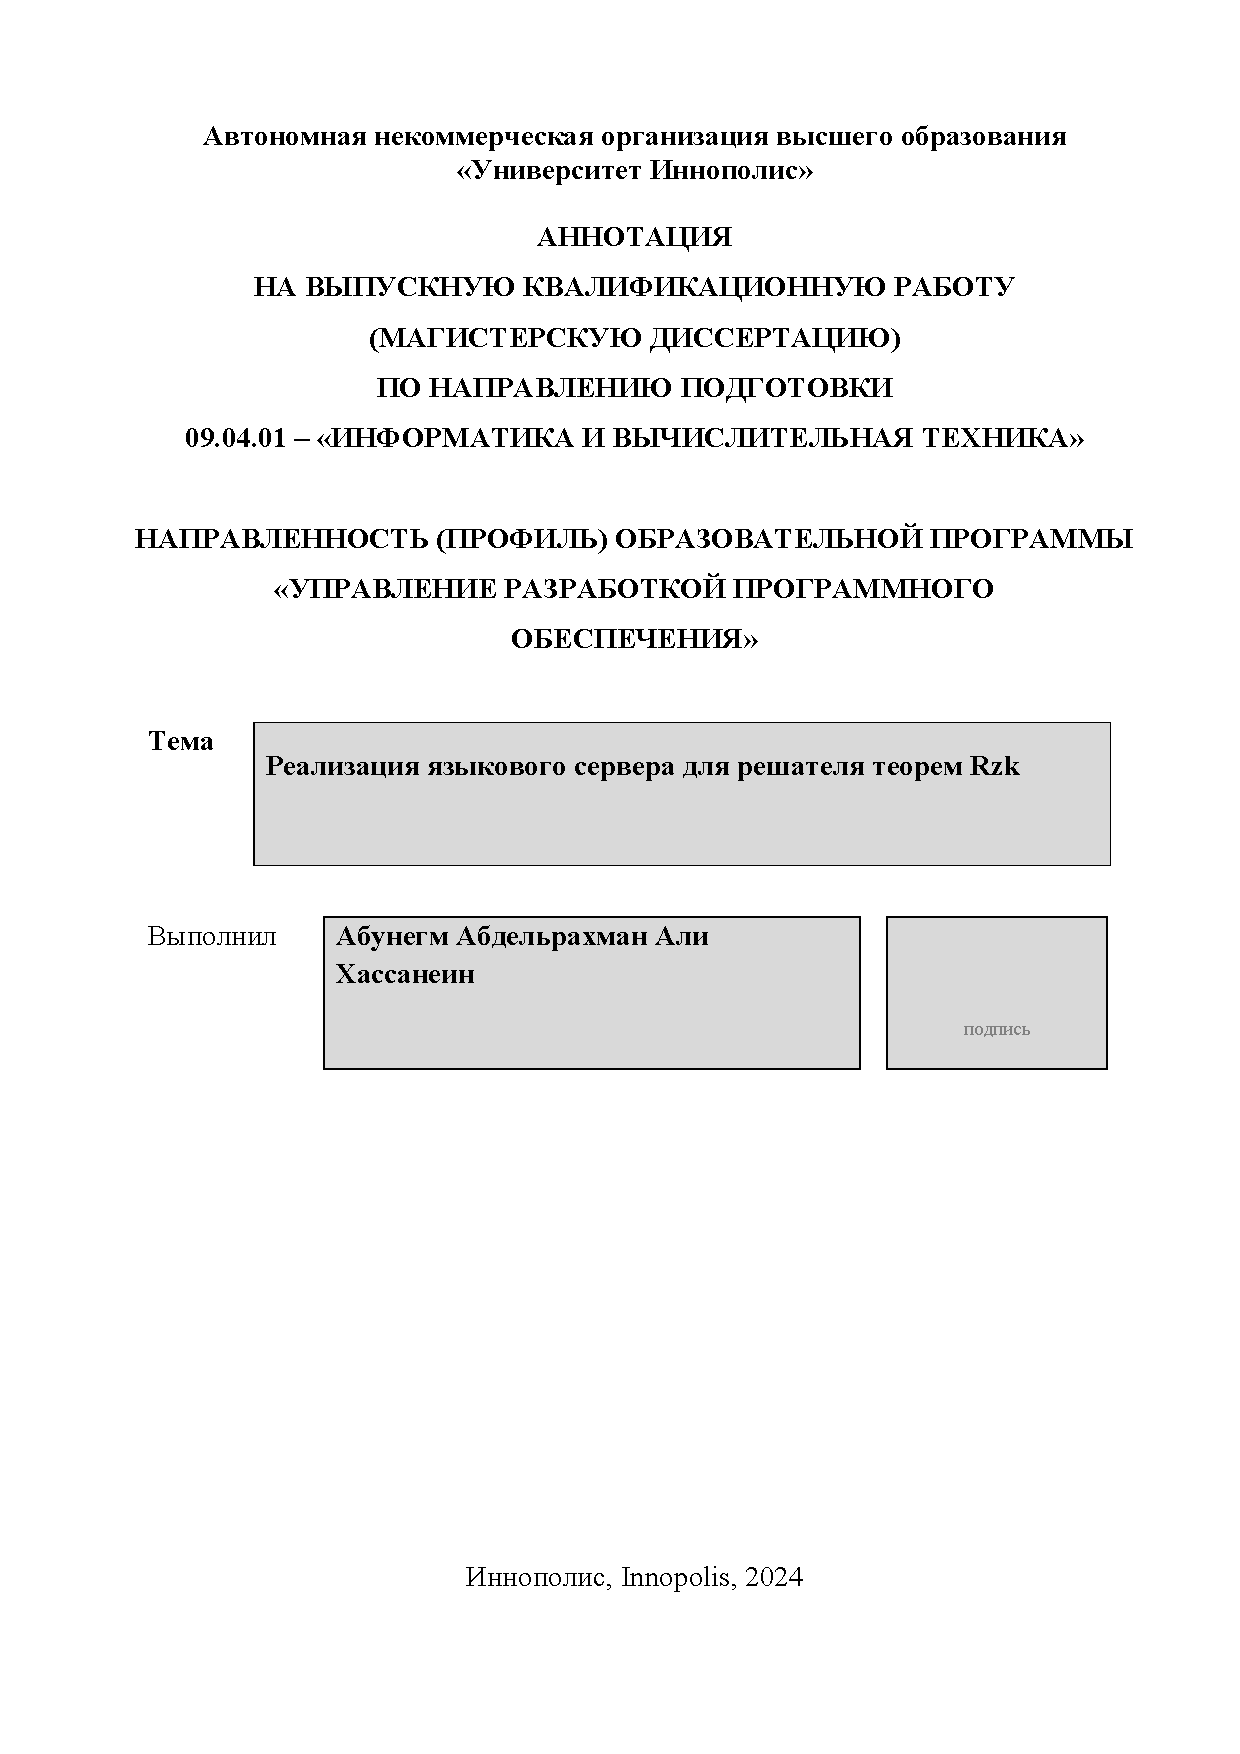
\includepdf[pages=-,offset={-\hoffset} {\voffset}]{annotation-title.pdf}

\newpage
\tableofcontents
\begin{abstract}
  % skip one line to make the abstract start with indent

  Теория типов Рила-Шулмана для синтетических $\infty$-категорий - это новая теория, основанная на теории типов гомотопий (HoTT).
  Экспериментальный помощник доказательств \Rzk{} предлагает автоматическую проверку доказательств для этой теории.
  С целью сделать эту теорию более доступной для математиков и компьютерных ученых,
  мы представляем работу по созданию набора командных и интерактивных инструментов для \Rzk{}.
  Эти инструменты включают сервер языка, расширение для Visual Studio Code (VS Code),
  и список небольших утилит для удобства.
  Хотя мы сосредоточены на поддержке VS Code,
  сервер языка также совместим с другими популярными редакторами, поддерживающими Language Server Protocol (LSP),
  такими как Emacs и Vim.
\end{abstract}

\setcounter{page}{4}
% set manually the number, from which Глава 1 starts!
% Why do we put 4 in this case?
% Title page - page 1
% Оглавление - page 2
% Аннотация - page 3
% Глава 1 - page 4
% In your annotation the counter number can be different, please count carefully and insert the corresponding number.

\chapter{Введение}
\label{chap:intro}

\section{Ассистенты доказательств}

Ассистенты доказательств, или интерактивные доказательные системы (ITP), используются в математике и компьютерных науках для проверки математических доказательств. Эти инструменты, такие как Agda~\cite{BoveDybjerNorell2009}, Coq~\cite{BertotCasteran2013} и Lean~\cite{deMouraUllrich2021}, помогают обеспечить корректность и надежность сложных утверждений и программных систем.

\Rzk{}~\cite{Kudasov2023-github-rzk} - новый ассистент доказательств на основе теории типов Рила-Шулмана для синтетических $\infty$-категорий~\cite{RiehlShulman2017, Riehl2023}. Этот экспериментальный ассистент использовался для формализации важных результатов для $\infty$-категорий, включая лемму Йонеды~\cite{Kudasov2023}. Однако ему не хватало интерактивных функций, таких как подсветка синтаксиса. В этой статье мы описываем реализацию утилит и инструментов для \Rzk{}, включая поддержку сервера языка и расширения для VS Code, чтобы улучшить взаимодействие с пользователем.

\section{Серверы языков}

С появлением новых редакторов кода возникала необходимость в поддержке разных языков программирования. Microsoft предложила стандартизировать протокол общения между редактором и сервером языка через Language Server Protocol (LSP) \cite{Gunasinghe2022}. Это позволяет разработчикам языка реализовать сервер один раз, получая поддержку в любом редакторе, поддерживающем LSP. Примеры функций языка включают диагностику, переход к определениям, автозаполнение, семантическую подсветку и др.

Этот протокол особенно полезен для интерактивных доказательных систем, которые зависят от удобства редактирования. Сервер языка выполняет функции проверки типов компиляторов, а также поддерживает больше функций, включая отображение переменных и пошаговое интерактивное доказательство.

\section{Вклад}

В этой статье описана реализация утилит и интерактивных инструментов для \Rzk{} с акцентом на сервер языка и расширение для VS Code. Основные вклады включают:
\begin{itemize}
  \item Сервер языка для \Rzk{}, поддерживающий основные функции LSP.
  \item Расширение для VS Code для загрузки и использования сервера языка.
  \item Форматтер кода для \Rzk{}.
  \item Плагин для MkDocs для рендеринга кода \Rzk{} в Markdown.
\end{itemize}

\chapter{Обзор литературы}
\label{chap:lr}

Это исследование основывается на работах в областях ассистентов доказательств, языковых серверов и архитектуры компиляторов на основе запросов. В этой главе рассматривается наиболее релевантная литература.

\section{Ассистенты доказательств}

\Rzk{}~\cite{kudasov2023experimental} основывается на последних разработках других ассистентов доказательств, предоставляя удобный интерфейс для синтетических $\infty$-категорий.

\subsection{Ассистенты доказательств для синтетических $\infty$-категорий}

\subsubsection{Coq}

Coq \cite{huet1997coq} является одним из первых ассистентов доказательств и поддерживает зависимые типы и индуктивные конструкции. Он используется в различных областях, включая формальную верификацию и теорию программирования. Библиотека UniMath \cite{DanielGrayson2024, MacPherson2019} добавляет поддержку Homotopy Type Theory и унивальных оснований.

\subsubsection{Cubical Agda}

Agda \cite{BoveDybjerNorell2009} — это ассистент доказательств, основанный на парадигме "доказательства как типы". Cubical Agda \cite{VEZZOSI2021} расширяет Agda кубической теорией типов, позволяя формализовать Homotopy Type Theory \cite{Cohen2016}.

\subsection{Библиотеки для разработки ассистентов доказательств}

\subsubsection{Proof General}

Proof General \cite{Aspinall2000} — это инструмент для разработки интерактивных доказательных систем на основе редактора Emacs. Он поддерживает множество известных ассистентов доказательств, таких как Coq и Isabelle.

\subsubsection{A.L.G.A.E.}

A.L.G.A.E. \footnote{\url{https://redprl.org/\#algae}} — это проект, предоставляющий библиотеки для разработки ассистентов доказательств на OCaml. Он включает инструменты для диагностики компилятора, уровней вселенных и поддержки кубической теории типов \cite{Kovacs2021}.

\section{Протокол языкового сервера}

Протокол языкового сервера (LSP) был разработан Microsoft для отделения реализации языка от интерфейса редактора \cite{Buender2019}. Он используется многими инструментами разработки, такими как Visual Studio Code, Emacs и Vim.

\subsection{Спецификация языкового серверного протокола}

LSP был разработан для языков общего назначения, но для спецификационных языков, таких как ассистенты доказательств, требуется расширение. Jonas Rask et al. \cite{JonasKjaerRask2021} предложили расширение LSP для спецификационных языков, называемое Specification Language Server Protocol (SLSP). Оно добавляет новые запросы и уведомления, а также вид для отображения информации о доказательствах.

\subsection{Расширение VS Code для Lean 4}

Основной способ разработки программ на Lean 4 — это использование расширения VS Code, которое предоставляет интерфейс для работы с Lean \cite{Nawrocki2023}. Это расширение использует LSP для связи с сервером Lean и предоставляет такие функции, как панель Info View.

\subsection{Отчеты о языковых серверах для ассистентов доказательств}

Несколько отчетов описывают разработку языковых серверов для ассистентов доказательств. Bour et al. \cite{Bour2018} описывают языковой сервер для OCaml, Kaliszyk \cite{Kaliszyk2007} предлагает архитектуру веб-интерфейсов для Coq, а Tavante \cite{Tavante2021} исследует инструменты для ассистентов доказательств.

\section{Архитектура компиляторов на основе запросов}

Традиционная компиляция состоит из пяти фаз \cite{dragon-book}: лексический анализ, синтаксический анализ, семантический анализ, генерация кода и оптимизация. Архитектура компиляторов на основе запросов \cite{ollef-rock} предназначена для интерактивных сред программирования, где каждая фаза представлена как независимый запрос. Эта архитектура более гибкая и позволяет кэшировать результаты запросов, что ускоряет интерактивные среды.

Недавние исследования показывают применение такой архитектуры в отладке объектно-ориентированных программ \cite{Lencevicius1997}. Lenkefi и Mezei \cite{icsoft22} разработали библиотеку для компиляторов на основе запросов и использовали её для реализации компилятора и языкового сервера для простого языка программирования.

Инкрементальный синтаксический анализ \cite{Ghezzi1979, diekmann2019editing, Wagner1998}, который обновляет синтаксическое дерево с изменениями исходного кода, также значительно ускоряет интерактивные компиляторы. Многие генераторы парсеров, такие как Tree-sitter \cite{tree-sitter} и Ohm \cite{Dubroy2017}, уже включают эту технологию.

\chapter{Системные требования и проектирование}
\label{chap:req}

\section{Требования}

Требования к ассистенту доказательств (и его расширению для VS Code) можно разделить на две категории: основные функции и функции для удобства пользователей. Основные функции — это необходимые функциональности и свойства, которые ассистент доказательств должен иметь для поддержки языкового сервера без особых трудностей. Функции для удобства пользователей не влияют на внутренний дизайн ассистента доказательств, но помогают обеспечить приятный пользовательский опыт.

\subsection{Основные функции}

Так как сам ассистент доказательств \Rzk{} уже находится в разработке и имеет работающий типизатор, основное внимание уделяется функциям, необходимым для использования ассистента доказательств в интерактивной среде. До сих пор ассистент доказательств имел только командный интерфейс (CLI), который проверял все входные файлы каждый раз, когда пользователь хотел проверить доказательство. Было очевидно, что это неустойчивый способ разработки доказательств, особенно для больших проектов.

К счастью, была четкая разделение между основным алгоритмом типизации и интерфейсом в виде библиотеки, что упростило работу по модификации только интерфейса без изменения алгоритма. Этот интерфейс должен поддерживать инкрементальную типизацию, что позволяет проверять только измененные части кода, значительно ускоряя процесс. Это похоже на функцию инкрементальной компиляции TypeScript, которая кэширует информацию во время каждой компиляции и компилирует только измененные файлы \cite{Vanderkam2024}.

Интерфейс должен уметь кэшировать результаты типизации в памяти и обновлять их по мере необходимости. Модуль кэширования должен поддерживать различные методы кэширования, такие как кэширование в памяти или на диске, поскольку могут быть разные пользовательские интерфейсы с разными требованиями (например, CLI против языкового сервера).

Возможность поддержки различных пользовательских интерфейсов важна, поскольку ассистент доказательств не ограничивается только VS Code. Потребителями ассистента доказательств могут быть не только люди, предпочитающие графический интерфейс, но и другие программные инструменты, такие как CI-пайплайны или другие вспомогательные инструменты. Поэтому также необходим командный интерфейс, позволяющий использовать ассистент доказательств в неинтерактивных условиях.

Наконец, интерфейс ассистента доказательств должен быть спроектирован таким образом, чтобы его легко можно было расширять и модифицировать, что обеспечивает короткий цикл разработки новых функций. Это особенно важно для ассистента доказательств, который все еще находится в разработке и имеет множество запланированных функций.

\subsection{Функции для удобства пользователей}

Основная цель описанных выше основных функций — помочь улучшить пользовательский опыт ассистента доказательств. Эти требования к UX не обязательно являются функциями или функциональностями, но также включают свойства, которые должен иметь ассистент доказательств.

Самое важное из этих свойств — простота использования для новичков (или непрограммистов) и интуитивно понятный интерфейс. Это критично для широкого распространения ассистента доказательств, так как целевая аудитория не обязательно опытные программисты. В любом случае, процесс редактирования должен быть удобным для любого пользователя.

Быстрая обратная связь по введенным данным — еще одно важное свойство, которое должен иметь ассистент доказательств. Это включает, например, диагностические сообщения, отображаемые сразу после ввода ошибки пользователем, а также информацию при наведении курсора, показывающую тип переменной и местоположение ее определения. Также включены автозавершение и предложения кода, которые помогают предотвратить использование неопределенных переменных. Пользователи также ожидают возможности перехода к определению переменной или поиска всех ссылок на нее.

Наконец, ожидаются функции, общие для большинства популярных IDE, такие как интеграция с git, отладка и инструменты рефакторинга.

\section{Проектирование}

С учетом вышеупомянутых требований ясно, что ассистент доказательств должен поддерживать языковой сервер. Кроме того, языковой сервер должен быть реализован с использованием LSP, чтобы обеспечить легкую интеграцию с различными редакторами без необходимости писать отдельное расширение или плагин для каждого текстового редактора. Ядро ассистента доказательств должно предоставлять интерфейс, который языковой сервер может использовать для взаимодействия с ним, а также CLI для неинтерактивного использования.

Сам языковой сервер будет реализован на Haskell, так как ассистент доказательств также написан на Haskell. Это позволит легко интегрировать его с ядром ассистента доказательств и упростит обслуживание кода.

Система может быть разделена на следующие компоненты: основной типизатор, CLI, языковой сервер, расширение для VS Code и утилиты. Основной алгоритм типизации — это сердце ассистента доказательств, отвечающее за проверку корректности доказательств; он выходит за рамки данного проекта, который предполагает его готовность и строится на его основе.

Затем идет интерфейс типизатора, который можно разделить на две части: CLI и языковой сервер. CLI — это простой интерфейс, позволяющий пользователю проверять файл или проект из командной строки. Он также полезен для неинтерактивного использования, такого как CI-пайплайны или другие инструменты. Его простота также делает его разумным интерфейсом для тестирования новых функций, так как здесь меньше подвижных частей.

Другой интерфейс — это языковой сервер, который отвечает за предоставление интерактивного интерфейса к ассистенту доказательств. Это более удобный из двух интерфейсов и будет использоваться большинством пользователей. Он реализован с использованием протокола Language Server от Microsoft для обеспечения легкой интеграции с различными текстовыми редакторами, такими как VS Code, Vim или Emacs. Языковой сервер также отвечает за предоставление функций, ожидаемых от современного языка программирования, таких как автозавершение, диагностические сообщения и информация при наведении.

Расширение для VS Code — это тонкая оболочка вокруг языкового сервера, которая помогает легко загружать копию языкового сервера и интегрировать его с VS Code. Оно делает это, проверяя страницу релизов в репозитории GitHub\footnote{\url{https://github.com/rzk-lang/rzk/releases}} и загружая последнюю соответствующую бинарную версию для операционной системы пользователя, которая затем кэшируется в локальном каталоге хранения расширения, предоставляемом VS Code. Расширение также упрощает сборку языкового сервера из исходников, если пользователь предпочитает это сделать. Дополнительно, оно предоставляет опцию указания пользовательского пути к языковому серверу для облегчения тестирования и разработки.

Расширение для VS Code доступно на нескольких платформах, включая Visual Studio Marketplace, Open VSX и GitHub. Это делается для того, чтобы расширение было легко обнаружимо пользователями и могло быть установлено из разных источников, особенно для пользователей, которые предпочитают не использовать проприетарное ПО Microsoft и вместо этого выбирают альтернативы, такие как VSCodium\footnote{\url{https://vscodium.com}}. VSCodium можно настроить для использования Open VSX в качестве своего рынка расширений, что позволяет пользователям устанавливать расширение оттуда. Наличие файла ".vsix" на странице релизов репозитория GitHub также способствует открытости и гибкости проекта и позволяет пользователям устанавливать расширение вручную, если они предпочитают это делать. Выпуск на все эти платформы автоматизирован с помощью GitHub Actions, который собирает расширение и загружает его на соответствующие платформы.

Наконец, разработаны вспомогательные инструменты для выполнения мелких задач, связанных с использованием ассистента доказательств. Например, есть плагин Python\footnote{\url{https://pypi.org/project/mkdocs-plugin-rzk/}} для MkDocs, который автоматизирует рендеринг SVG файлов в проекте формализации, использующем MkDocs, что полезно для рендеринга топов в результатирующей документации. Другой инструмент — это GitHub Action\footnote{\url{https://github.com/rzk-lang/rzk-action}}, упрощающий процесс установки \Rzk{} в CI-пайплайне и запуска его на файлах проекта.

\chapter{Реализация}
\label{chap:impl}

\section{Языковой сервер \Rzk{} и расширение для VS Code}

Описываем реализацию языкового сервера и расширения для \Rzk{} в среде VS Code.
Языковой сервер имеет прямой доступ к внутренностям доказательного ассистента,
включая алгоритм проверки типов и внутреннее абстрактное синтаксическое представление,
и предоставляет интерфейс, соответствующий протоколу языкового сервера.
Расширение для VS Code действует как посредник между редактором и языковым сервером,
предоставляя интерактивные возможности пользователю.

\subsection{Особенности}

Мы рассматриваем поддержку языкового сервера следующих особенностей.

\subsubsection{Интуитивный интерфейс и подсветка синтаксиса}

Расширение для VS Code предлагает интуитивно понятный интерфейс,
соответствующий ожиданиям математиков и компьютерных учёных.
Пользователи получают ясную и доступную навигацию,
позволяющую эффективно исследовать структуры, основанные на HoTT.
Кроме того, расширение обеспечивает подсветку синтаксиса и семантики,
улучшая читаемость кода и облегчая обнаружение ошибок.

\begin{figure}[ht]
  \centering
  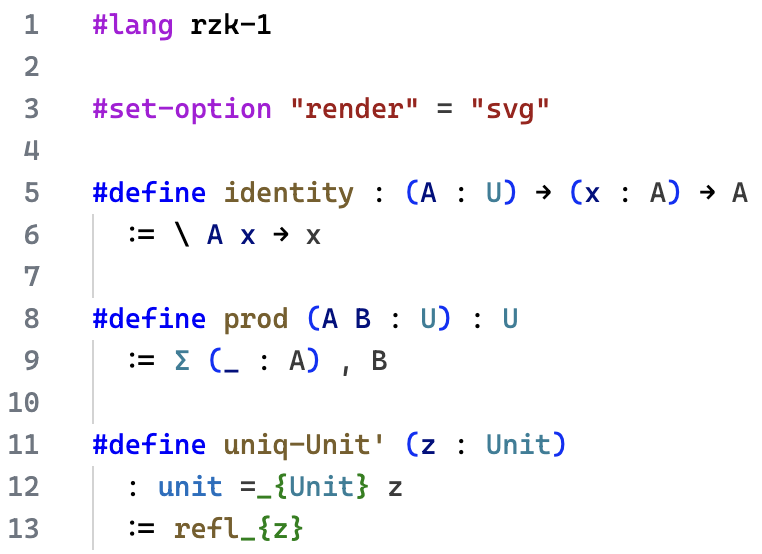
\includegraphics[width=0.7\textwidth]{figs/syntax-highlighting.png}
  \caption{Подсветка синтаксиса/семантики в VS Code.}
  \label{figure:syntax-highlighting}
\end{figure}

\subsubsection{Автодополнение кода и предложения}

Расширение для VS Code \Rzk{} использует LSP для предложения интеллектуального
автодополнения кода и предложений, основанных на контексте. В процессе работы
с \Rzk{} расширение помогает писать код более эффективно, предоставляя
соответствующие предложения, снижая вероятность синтаксических ошибок и
ускоряя процесс разработки.

\subsection{Расширение для VS Code}

Для предоставления пользователю указанных функций необходимо использовать тонкий обёртку вокруг языкового сервера в виде расширения для VS Code. Дополнительно расширение управляет установкой самого языкового сервера на всех основных операционных системах (Windows, macOS и Ubuntu) с использованием предварительно собранных бинарных файлов, прикреплённых к релизам на GitHub, а также обеспечивает сборку языкового сервера из исходного кода на платформах, для которых предварительно собранные бинарные файлы недоступны. Исходный код расширения доступен в репозитории GitHub\footnote{\url{https://github.com/rzk-lang/vscode-rzk}}, а само расширение доступно на платформе Visual Studio Marketplace\footnote{\url{https://marketplace.visualstudio.com/items?itemName=NikolaiKudasovfizruk.rzk-1-experimental-highlighting}} и на реестре Open VSX\footnote{\url{https://open-vsx.org/extension/NikolaiKudasovfizruk/rzk-1-experimental-highlighting}}, а также предварительно собранный бинарный файл на странице релизов GitHub\footnote{\url{https://github.com/rzk-lang/vscode-rzk/releases}}.

\subsubsection{Установка и активация}

После активации расширение проверяет доступность исполняемого файла \Rzk{} в переменной среды \texttt{PATH} системы. Если файл недоступен, расширение проверяет наличие загруженного ранее бинарного файла в локальном хранилище расширения. Если ни то, ни другое не найдены, пользователю предлагается скачать последнюю совместимую версию бинарного файла с страницы релизов GitHub и сохранить его в локальном хранилище. Пользователь может изменить это поведение, указав пользовательский путь к бинарному файлу языкового сервера.

Для загрузки предварительно собранного бинарного файла \Rzk{} расширение запрашивает доступные релизы на GitHub и находит последний релиз, совместимый с установленной версией расширения. Совместимость определяется с помощью диапазона версий в семантическом формате\cite{Preston2013semantic}, заданном в исходном коде расширения, и используется для фильтрации релизов и поиска последнего, удовлетворяющего заданному диапазону.

Затем расширение загружает бинарный файл с помощью SDK Octokit и извлекает tar-архив в локальное хранилище. После этого расширение просто запускает языковой сервер в отдельном процессе и устанавливает соединение с ним, остальное обрабатываются VS Code и языковой сервером.

\subsubsection{Настройка}

Расширение предоставляет пользователю опции конфигурации для настройки поведения расширения. Пользователь может указать путь к исполняемому файлу \Rzk{}, что полезно для пользователей, у которых исполняемый файл установлен в нестандартном местоположении, а также для тестирования. Пользователь также может включить или отключить функцию форматирования и выбрать, получать ли предварительные версии \Rzk{}.

Это достигается с помощью поля конфигурации\footnote{\url{https://code.visualstudio.com/api/references/contribution-points\#contributes.configuration}} в файле \texttt{package.json} расширения.

\subsection{Языковой сервер \Rzk{}}

В центре инструментального комплекса \Rzk{} находится языковой сервер, который обеспечивает все функции редактора, сделав разработку доказательств в \Rzk{} приятной. В настоящее время он поддерживает семантическую подсветку, диагностические сообщения и автодополнение текста. Также в разработке находится функция отчётности о ходе длительных процессов (например, проверка типов для больших проектов).

Первоначально языковой сервер поставляется вместе с доказательным ассистентом \Rzk{} как отдельная подкоманда, но планируется разделение этих компонентов и зависимость языкового сервера от основной библиотеки. Они реализованы на языке программирования Haskell с использованием пакета \texttt{lsp}\footnote{\url{https://hackage.haskell.org/package/lsp}}.

Эта точка входа становится доступной пользователю как отдельная подкоманда, \texttt{rzk lsp}, которая запускает языковой сервер и ожидает входящих соединений от редактора. Он определяет обработчики сообщений LSP и инициализирует сервер с необходимой конфигурацией для синхронизации между файлами в редакторе и языковым сервером.

Стратегически важно отметить, что языковой сервер разработан с учётом совместимости не только с VS Code, но и с

\chapter{Оценка и обсуждение}
\label{chap:eval}

\section{Оценка}

Обратная связь по \Rzk{} и его языковому серверу была собрана через прямое взаимодействие с пользователями и сравнение с другими доказательными помощниками. Пользователи выразили удовлетворение новыми функциями и улучшенным пользовательским опытом. Хотя сервер развивается и не имеет некоторых функций, присутствующих в других серверах, он удовлетворяет базовым требованиям и полезен на практике.

\subsection{Летняя школа ITP 2023}

Основной отзывы пользователей были собраны на летней школе по взаимодействию доказательных помощников и математики в 2023 году в Регенсбурге, Германия. Участники получили обучение по \Rzk{}, и отзывы были собраны через неформальные обсуждения. Запросы на функции и исправления были замечены и решены быстро, включая отзывы от экспертов по теории типов.

\subsection{Проекты формализации}

\Rzk{} был применен в нескольких сообщественных проектах по формализации, оценивающих удобство сопутствующих инструментов, таких как языковой сервер и расширение для VS Code. Заметные проекты включают \textbf{sHoTT}, \textbf{HoTT Book} и \textbf{Yoneda}, фокусирующиеся на симплициальной гомотопической теории типов, теоремах гомотопической теории типов и сравнительных формализациях леммы Йонеды.

\section{Обсуждение и рефлексия}

\Rzk{} поддерживает математиков и компьютерных ученых, изучающих высшую категориальную теорию и гомотопическую теорию типов. Несмотря на скромное количество пользователей, отзывы показывают значительное улучшение опыта редактирования. В будущем планируется внедрение автоматизированных инструментов тестирования, формальных исследований пользователей и дополнительных функций LSP для более гладкого редактирования.

\chapter{Заключение}
\label{chap:conclusion}

\section{Резюме}

Мы разработали и реализовали начальный прототип языкового сервера и расширения для VS Code для экспериментального доказательного помощника \Rzk{}. Промежуточные результаты этой работы были представлены на школе \textit{Взаимодействие доказательных помощников и математики}\footnote{\url{https://itp-school-2023.github.io/}} в Германии в сентябре 2023 года. Это помогло собрать обратную связь от пользователей и реагировать на неё непосредственно. Мы уверены, что текущие пользователи в основном удовлетворены прототипом инструментов, но также предоставили полезные предложения для дальнейшего улучшения.

\section{Планы на будущее}

Текущая реализация языкового сервера для \Rzk{} находится на ранних стадиях. Есть множество отсутствующих функций и мест для улучшения. Например, необходимо провести формальное исследование эффективности продукта этой работы с помощью опроса пользователей для выявления наиболее важных функций для работы.

В будущем мы планируем поддержку отображения информации о переменных при наведении, переход к определению, переименование символов и другие полезные функции LSP. Также планируется поддержка отображения топов как изображений и добавление информационного веб-представления, аналогичного тому, которое предоставляет Lean 4 \cite{Nawrocki2023}.

Также ожидается, что из этого проекта вырастет библиотека на Haskell для разработки языковых серверов (особенно для доказательных помощников).



\printbibliography[heading=bibintoc,title={Список использованной литературы}]
\end{document}
